\documentclass{article}
\usepackage[spanish]{babel}
\usepackage[utf8]{inputenc}

\title{La gestión en contabilidad}
\author{Jose Miguel Porozo \and Tafur Issa}
\date{23 de agosto de 2023}

\begin{document}

\maketitle

\section{Introducción}
La gestión contable es un componente esencial en cualquier organización, ya que implica el seguimiento, registro y análisis de las transacciones financieras para garantizar la salud financiera y la toma de decisiones. En la era digital actual, la gestión contable ha evolucionado hacia el uso de bases de datos, permitiendo un almacenamiento eficiente y accesible de información financiera. Las bases de datos son una herramienta fundamental, ya que nos permite acceder a nuestros registros contables de manera rápida y también ofrecen ciertos niveles de seguridad para nuestros registros contables, evitando que la información sea modificada o vista por fuentes externas a la organización o empresa.

\section{Objetivo General}
El objetivo principal de este artículo es analizar en profundidad la gestión de contabilidad como un componente crítico en la administración financiera y la toma de decisiones empresariales, y explorar cómo la tecnología y los subsistemas contribuyen a optimizar este proceso. Además, se busca resaltar la importancia de la seguridad de los datos en el entorno de gestión de contabilidad y presentar medidas clave para proteger la información financiera.

\subsection{Objetivos Específicos}
\begin{enumerate}
    \item Evaluar la Efectividad de las Bases de Datos en la Gestión Contable: Analizar cómo el uso de bases de datos en la gestión contable mejora la accesibilidad, almacenamiento y seguridad de los registros financieros.
    
    \item Identificar los Beneficios de la Digitalización en la Gestión Contable: Investigar cómo la digitalización ha impactado positivamente en la eficiencia, la toma de decisiones y la precisión de los registros contables.
    
    \item Analizar la Seguridad de la Información Financiera en las Bases de Datos Contables: Evaluar las medidas de seguridad implementadas en las bases de datos contables para proteger la información financiera contra accesos no autorizados y modificaciones indebidas.
    \newpage


\begin{figure}[h]
    \centering
    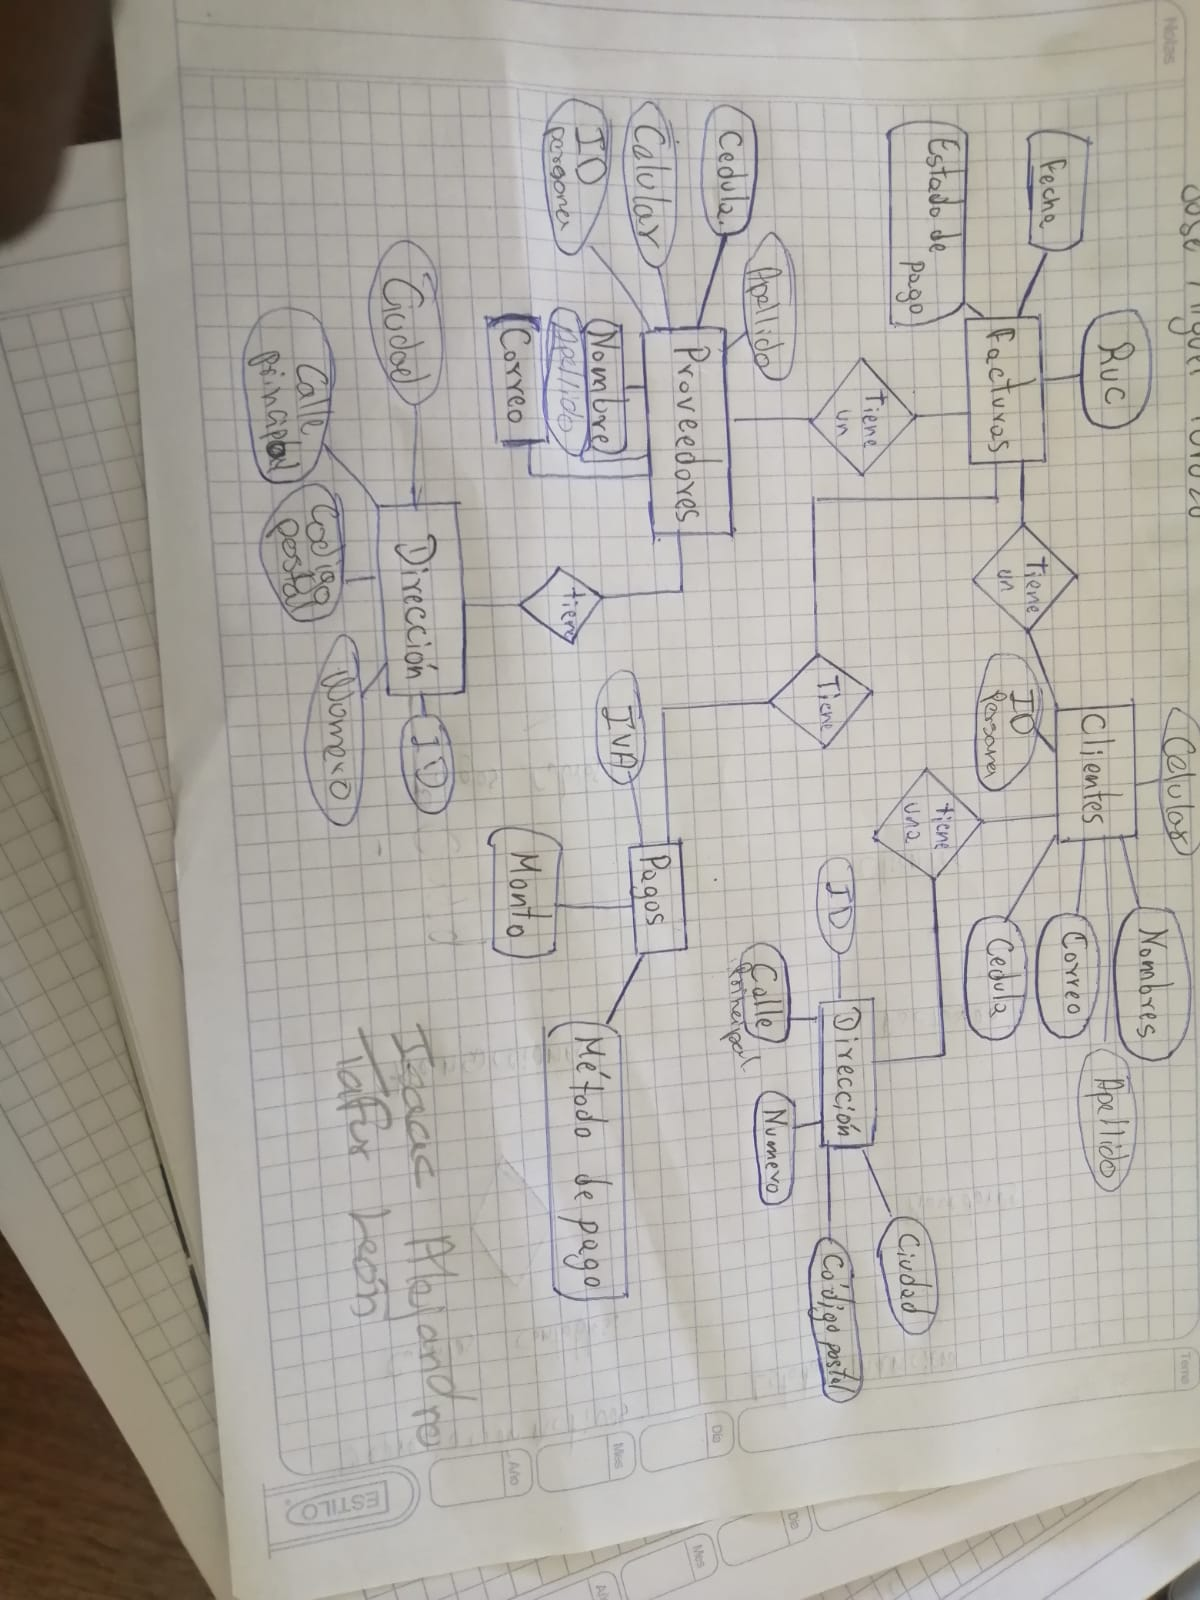
\includegraphics[width=1.7\textwidth, angle=90]{Contabilidad.jpg}
    \caption{Diagrama}
    \label{fig:img01}
\end{figure}

\end{enumerate}
\end{enumerate}

\end{document}
